\section{qfileiconview.cpp File Reference}
\label{qfileiconview_8cpp}\index{qfileiconview.cpp@{qfileiconview.cpp}}


{\tt \#include \char`\"{}qfileiconview.h\char`\"{}}\par
{\tt \#include $<$qpainter.h$>$}\par
{\tt \#include $<$qstringlist.h$>$}\par
{\tt \#include $<$qpixmap.h$>$}\par
{\tt \#include $<$qmime.h$>$}\par
{\tt \#include $<$qstrlist.h$>$}\par
{\tt \#include $<$qdragobject.h$>$}\par
{\tt \#include $<$qmessagebox.h$>$}\par
{\tt \#include $<$qevent.h$>$}\par
{\tt \#include $<$qpopupmenu.h$>$}\par
{\tt \#include $<$qcursor.h$>$}\par
{\tt \#include $<$qapplication.h$>$}\par
{\tt \#include $<$qwmatrix.h$>$}\par
{\tt \#include $<$math.h$>$}\par
{\tt \#include $<$stdlib.h$>$}\par
{\tt \#include $<$kdebug.h$>$}\par


Include dependency graph for qfileiconview.cpp:\begin{figure}[H]
\begin{center}
\leavevmode
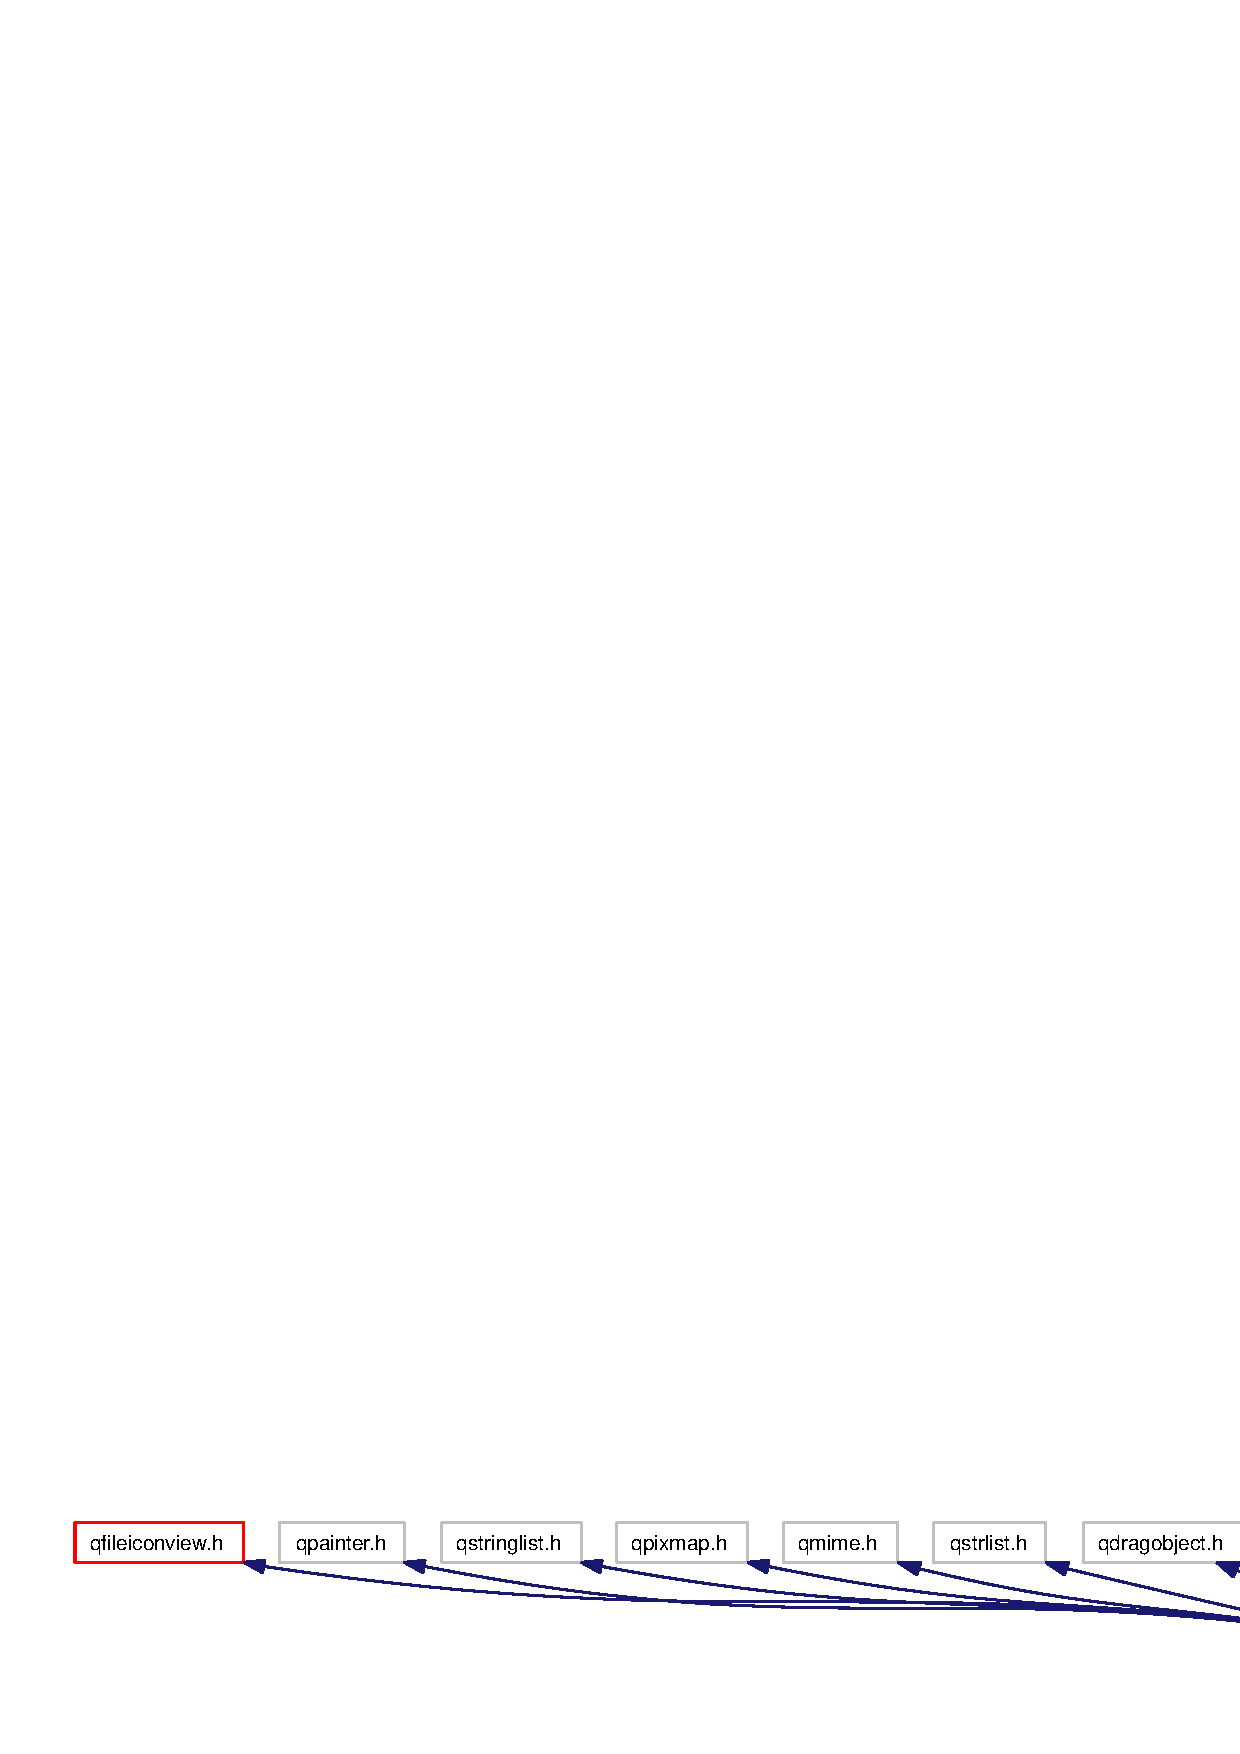
\includegraphics[width=420pt]{qfileiconview_8cpp__incl}
\end{center}
\end{figure}
\subsection*{Functions}
\begin{CompactItemize}
\item 
void {\bf cleanup} ()
\item 
QPixmap $\ast$ {\bf add\-Border} (QPixmap $\ast$pix, bool has\-Alpha)
\item 
bool {\bf is\-Root} (const QString \&s)
\end{CompactItemize}
\subsection*{Variables}
\begin{CompactItemize}
\item 
QPixmap $\ast$ {\bf icon\-File\-Large} = 0
\item 
QPixmap $\ast$ {\bf Array\-Image} [100]
\end{CompactItemize}


\subsection{Function Documentation}
\index{qfileiconview.cpp@{qfileiconview.cpp}!addBorder@{addBorder}}
\index{addBorder@{addBorder}!qfileiconview.cpp@{qfileiconview.cpp}}
\subsubsection{\setlength{\rightskip}{0pt plus 5cm}QPixmap$\ast$ add\-Border (QPixmap $\ast$ {\em pix}, bool {\em has\-Alpha})}\label{qfileiconview_8cpp_a3}




Definition at line 183 of file qfileiconview.cpp.

Referenced by Qt\-File\-Icon\-View\-Item::Qt\-File\-Icon\-View\-Item().



\footnotesize\begin{verbatim}184 {
185         //DAVID Read Background
186         QPixmap pbgxpm=QPixmap("/root/kde_application/hdass08/skin/bgxpm.png");
187         //DAVID Read Boarder Image
188         QImage ptop=QImage("/root/kde_application/hdass08/skin/border.png");
189         
190         //DAVID New a QPixmap res with size pix->size()
191         QPixmap res(pix->size());
192         
193         //Draw it on painter
194         QPainter p(&res);
195                 if(hasAlpha) 
196                         p.drawTiledPixmap (0, 0, pix->width(), pix->height(),pbgxpm);
197                 //DAVID draw broder to painter          
198                 p.drawImage(0, 0, ptop.scale(pix->width(), pix->height()));
199                 p.drawImage((int)floor((float)pix->width()/ptop.width()*14),
200                         (int)floor((float)pix->height()/ptop.height()*13),
201                         pix->convertToImage().smoothScale(
202                                 (int)ceil(pix->width()*0.79738562092),
203                                 (int)ceil(pix->height()*0.76691729323)));
204         p.end();
205         QImage a=res.convertToImage().scale(70,70);
206         QPixmap *temp=new QPixmap(a);
207         return temp;
208 }
\end{verbatim}\normalsize 
\index{qfileiconview.cpp@{qfileiconview.cpp}!cleanup@{cleanup}}
\index{cleanup@{cleanup}!qfileiconview.cpp@{qfileiconview.cpp}}
\subsubsection{\setlength{\rightskip}{0pt plus 5cm}void cleanup ()\hspace{0.3cm}{\tt  [static]}}\label{qfileiconview_8cpp_a2}




Definition at line 30 of file qfileiconview.cpp.

References icon\-File\-Large.

Referenced by Qt\-File\-Icon\-View::Qt\-File\-Icon\-View().



\footnotesize\begin{verbatim}31 {
32     
33     delete iconFileLarge;
34     iconFileLarge = 0;
35     
36 }
\end{verbatim}\normalsize 
\index{qfileiconview.cpp@{qfileiconview.cpp}!isRoot@{isRoot}}
\index{isRoot@{isRoot}!qfileiconview.cpp@{qfileiconview.cpp}}
\subsubsection{\setlength{\rightskip}{0pt plus 5cm}bool is\-Root (const QString \& {\em s})\hspace{0.3cm}{\tt  [static]}}\label{qfileiconview_8cpp_a4}




Definition at line 354 of file qfileiconview.cpp.

Referenced by Qt\-File\-Icon\-View::read\-Dir().



\footnotesize\begin{verbatim}355 {
356 #if defined(Q_OS_UNIX)
357     if ( s == "/" )
358         return TRUE;
359 #elif defined(Q_OS_WIN32)
360     QString p = s;
361     if ( p.length() == 3 &&
362          p.right( 2 ) == ":/" )
363         return TRUE;
364     if ( p[ 0 ] == '/' && p[ 1 ] == '/' ) {
365         int slashes = p.contains( '/' );
366         if ( slashes <= 3 )
367             return TRUE;
368         if ( slashes == 4 && p[ (int)p.length() - 1 ] == '/' )
369             return TRUE;
370     }
371 #endif
372 
373     return FALSE;
374 }
\end{verbatim}\normalsize 


\subsection{Variable Documentation}
\index{qfileiconview.cpp@{qfileiconview.cpp}!ArrayImage@{ArrayImage}}
\index{ArrayImage@{ArrayImage}!qfileiconview.cpp@{qfileiconview.cpp}}
\subsubsection{\setlength{\rightskip}{0pt plus 5cm}QPixmap$\ast$ {\bf Array\-Image}[100]}\label{qfileiconview_8cpp_a1}




Definition at line 29 of file qfileiconview.cpp.

Referenced by Qt\-File\-Icon\-View\-Item::pixmap(), and Qt\-File\-Icon\-View\-Item::Qt\-File\-Icon\-View\-Item().\index{qfileiconview.cpp@{qfileiconview.cpp}!iconFileLarge@{iconFileLarge}}
\index{iconFileLarge@{iconFileLarge}!qfileiconview.cpp@{qfileiconview.cpp}}
\subsubsection{\setlength{\rightskip}{0pt plus 5cm}QPixmap$\ast$ {\bf icon\-File\-Large} = 0\hspace{0.3cm}{\tt  [static]}}\label{qfileiconview_8cpp_a0}




Definition at line 28 of file qfileiconview.cpp.

Referenced by cleanup(), Qt\-File\-Icon\-View\-Item::pixmap(), and Qt\-File\-Icon\-View::Qt\-File\-Icon\-View().